% Appendix A

\chapter{Appendix A: Database schema} % Main appendix title

\label{AppendixA} % For referencing this appendix elsewhere, use \ref{AppendixA}

The database schema used to store the raw data collected from the software repositories studied is
documented in figure \ref{fig:appA_db_schema}.

\begin{figure}[H]
  \centering
  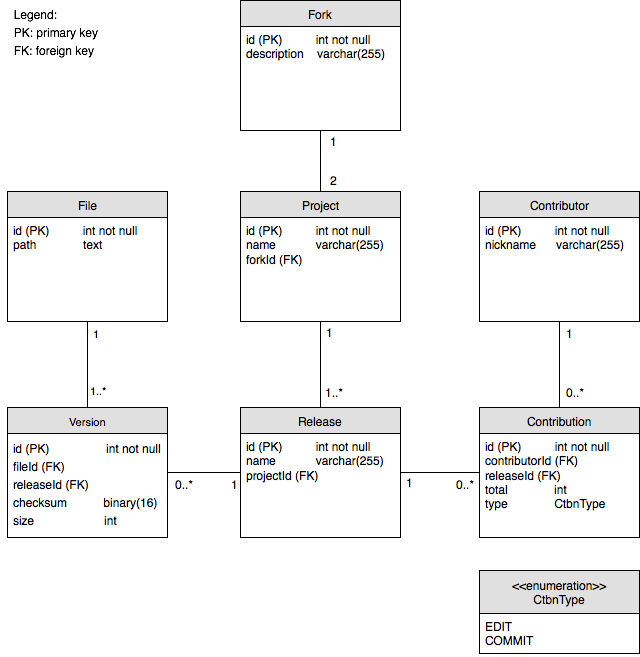
\includegraphics[width=\textwidth]{appA_db_schema.png}
  \caption{Database schema to hold data on forked repositories.}
  \label{fig:appA_db_schema}
\end{figure}


The database is composed of the following entities:
\begin{itemize}
  \item{One \textbf{fork} per \textbf{forked project} (e.g. MySQL, MariaDB).}
  \item{Each \textbf{project} has several \textbf{releases} (e.g. MySQL 5.5, MariaDB 10.0 ...).}
  \item{Each release is composed of \textbf{versions} of \textbf{files}, e.g. the file /src/main.c may be present or absent in a given release.}
  \item{Code churn characteristics (3.1.1) are recorded for each file \textbf{version}.}
  \item{Team characteristics (3.1.1) are recorded for each \textbf{release} as the number of
\textbf{contributions} (edits and commits) per \textbf{contributor}.}
\end{itemize}